\newpage
\section{Tạo Cơ sở dữ liệu}
\subsection{Tạo bảng}
\textbf{Yêu cầu:}
Viết các câu lệnh hiện thực các bảng dữ liệu đã thiết kế. Sinh viên phải tự xác định kiểu dữ liệu, kích thước dữ liệu và các ràng buộc (dựa trên mô tả nghiệp vụ và EERD ở Assignment 1). Các loại ràng buộc tối thiểu cần có:
\begin{itemize}
\item Khoá chính có dạng số nguyên tăng dần. Ví dụ: 1, 2, 3…
\item Khoá chính có dạng [PREFIX][Số tăng dần có X ký số]. Ví dụ EMP00001, EMP00002,…
\item Ràng buộc duy nhất 
\item Ràng buộc khoá ngoại
\item Ràng buộc not null 
\item Ràng buộc kiểm tra miền trị liên quan đến một cột hoặc nhiều cột. Ví dụ, mã phòng ban nằm trong khoảng [0, 20], thời gian check in phải nhỏ hơn thời gian check out,…
\end{itemize}

\textbf{Hiện thực}
\begin{lstlisting}[language=SQL, caption=Tạo bảng Product] 
CREATE TABLE `batch_product`.`product` (
  `ID` int NOT NULL AUTO_INCREMENT,
  `Name` varchar(16) NOT NULL,
  `Description` varchar(1024) NOT NULL,
  `Origin` varchar(32) NOT NULL,
  `Tag` varchar(16) DEFAULT 'OTHER',
  `Storage_Condition` varchar(1024) DEFAULT NULL,
  `Country of origin` varchar(16) DEFAULT NULL,
  `Price` decimal(10,2) NOT NULL,
  `Directions for use` varchar(1024) NOT NULL,
  `Certificate` varchar(512) DEFAULT NULL,
  `Warning` varchar(512) DEFAULT NULL,
  `Intended User` varchar(128) DEFAULT NULL,
  `Total amount from batch` int DEFAULT '0',
  PRIMARY KEY (`ID`),
  UNIQUE KEY `Name` (`Name`),
  CONSTRAINT `product_chk_1` CHECK ((`Total amount from batch` >= 0))
)
\end{lstlisting}

\begin{lstlisting}[language=SQL, caption=Tạo bảng Employee] 
CREATE TABLE `employee` (
  `ID` int NOT NULL AUTO_INCREMENT,
  `Name` varchar(16) NOT NULL,
  `Address` varchar(64) DEFAULT NULL,
  `Account` varchar(32) DEFAULT NULL,
  `Password` varchar(16) DEFAULT NULL,
  `Phone_no` varchar(16) DEFAULT NULL,
  `WorkingType` varchar(64) DEFAULT NULL,
  `JobType` enum('pharmacist','inventory manager','product manager','admin') DEFAULT NULL,
  `Credential` varchar(128) DEFAULT NULL,
  PRIMARY KEY (`ID`),
  UNIQUE KEY `ID_UNIQUE` (`ID`),
  UNIQUE KEY `Phone_no_UNIQUE` (`Phone_no`)
)
\end{lstlisting}
\subsection{Insert vào bảng}

\begin{lstlisting}[language=SQL, caption= Thêm data vào table product] 
INSERT INTO `batch_product`.`product` (
    `Name`, 
    `Description`, 
    `Origin`, 
    `Tag`, 
    `Storage_Condition`, 
    `Country of origin`, 
    `Price`, 
    `Directions for use`, 
    `Certificate`, 
    `Warning`, 
    `Intended User`, 
    `Total amount from batch`
)
VALUES
('Vitamin D', 
 'Vitamin D supplements the immune system.', 
 'USA', 
 'VITAMIN', 
 'Store in a dry place, away from direct sunlight.', 
 'United States', 
 15.99, 
 'Take 1 tablet/day after meal.', 
 'FDA Approved', 
 'Not for use by persons under 6 years of age.', 
 'Adult', 
 100);
\end{lstlisting}

\begin{lstlisting}[language=SQL, caption= Thêm data vào table employee] 
 INSERT INTO `employee_prescription`.`employee` (
    `Name`, 
    `Address`, 
    `Account`, 
    `Password`, 
    `Phone_no`, 
    `WorkingType`, 
    `JobType`, 
    `Credential`
)
VALUES
('John Doe', 
 '123 Main St, New York, NY', 
 'johndoe123', 
 'pass1234', 
 '1234567890', 
 'Full-time', 
 'pharmacist', 
 'Pharmacist License A12345');
\end{lstlisting}



\subsection{Auto-export Script}
Ta dùng phần mềm MySQL Workbench để thực hiện lấy script của tất cả cấu trúc bảng, data, procedure, trigger.

Trong MySQL Workbench, sau khi kết nối với database cần export, ta chọn Server > Data Export
\begin{figure}[h!]
    \centering
    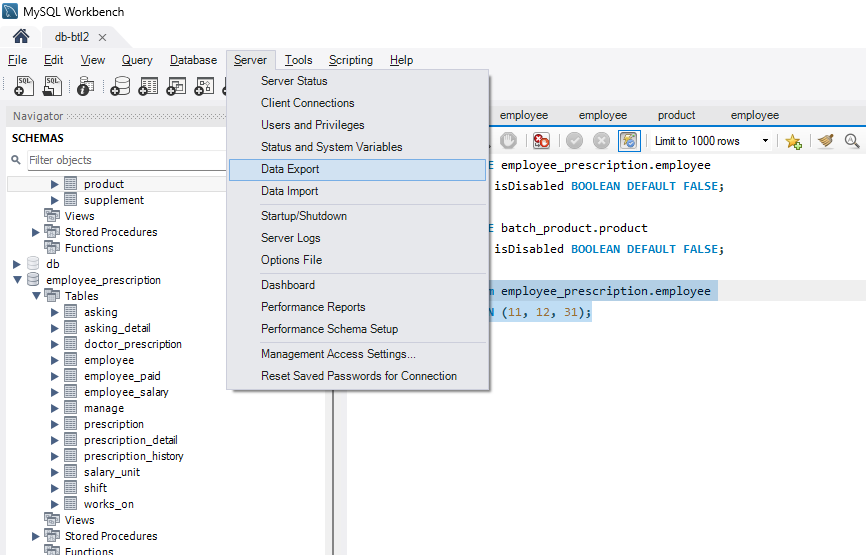
\includegraphics[scale=0.4]{Images/1.png}
    \caption{Chọn Data Export}
    % \label{fig:enter-label}
\end{figure}

Ta có một số các lựa chọn:
\begin{itemize}
    \item Tables to Export: Chọn các schema mà ta muốn export
    \item Objects to Export: Chọn có xuất các Procedures và Functions; Events; hoặc Triggers
    \item Export Options: Chọn xuất ra nhiều file hoặc một file, vị trí xuất file, ...
\end{itemize}
Sau khi tùy chọn xong, ta bấm Start Export
\begin{figure}[h!]
    \centering
    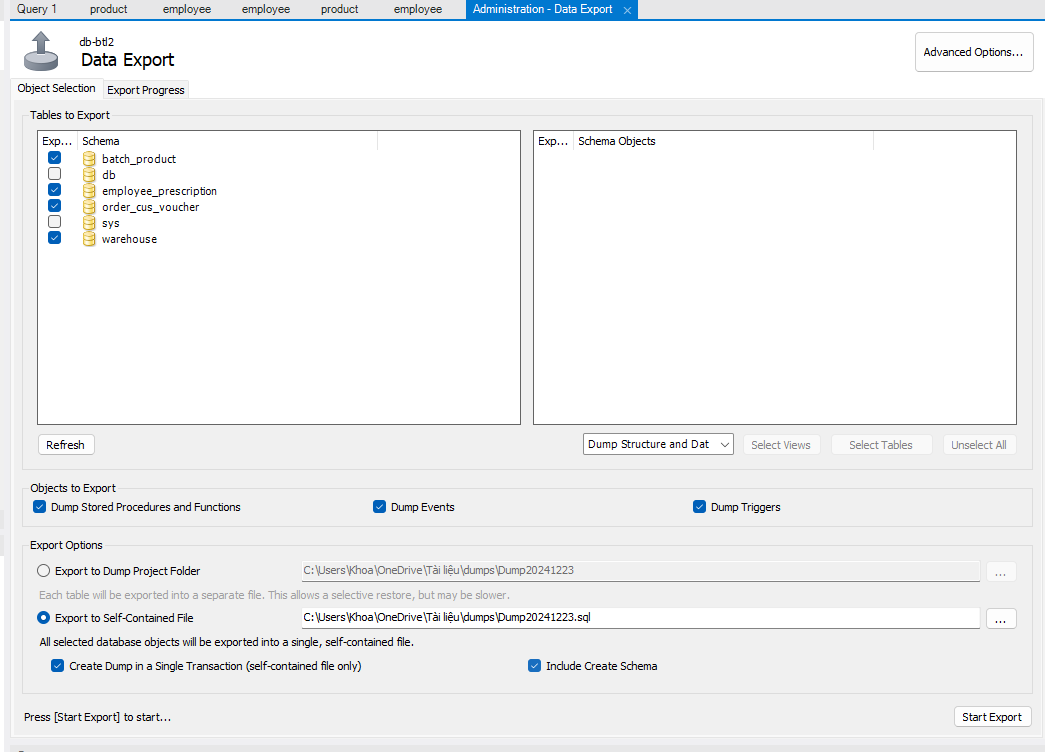
\includegraphics[scale=0.4]{Images/2.png}
    \caption{Màn hình chọn các tùy chọn để export}
    % \label{fig:enter-label}
\end{figure}

\newpage
Sau khi nhấn Start Export, ta sẽ được điều hướng đến màn hình này:
\begin{figure}[H]
    \centering
    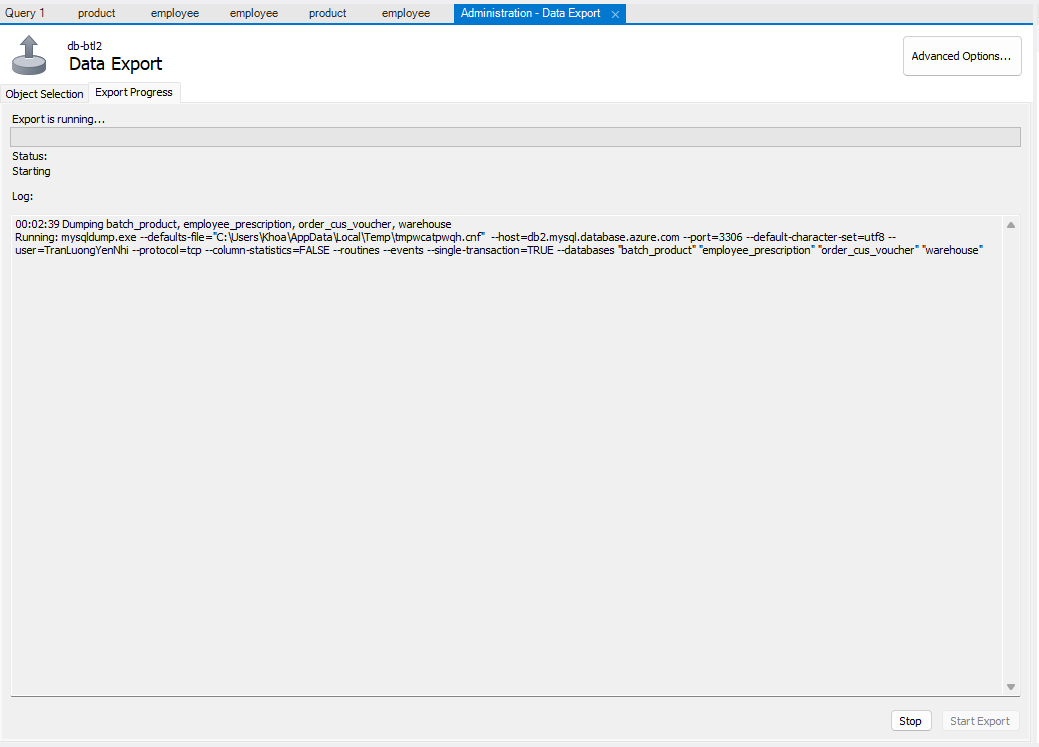
\includegraphics[scale=0.3]{Images/3.png}
    \caption{Màn hình trạng thái export}
    % \label{fig:enter-label}
\end{figure}


Đây là màn hình đó sau khi xong
\begin{figure}[H]
    \centering
    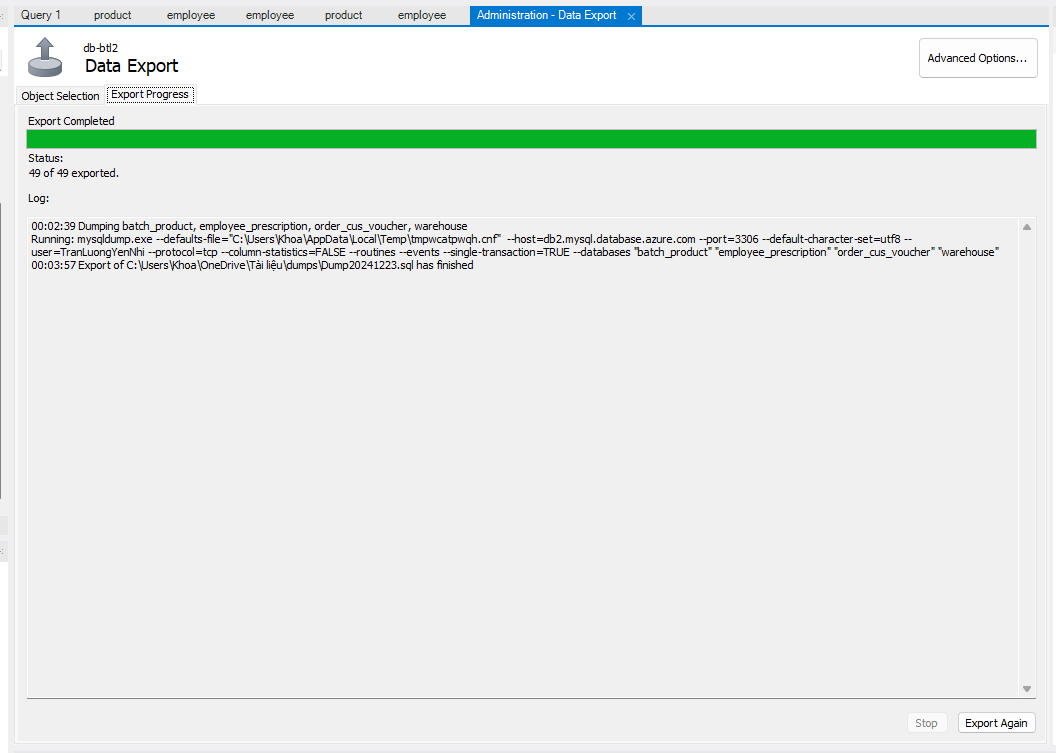
\includegraphics[scale=0.3]{Images/4.png}
    \caption{Màn hình hoàn thành export}
    % \label{fig:enter-label}
\end{figure}